\documentclass[conference]{IEEEtran}
\IEEEoverridecommandlockouts
% IEEEoverridecommandlockouts is needed only to identify funding in the first footnote.
% If funding acknowledgment is not needed, this line may be commented out.

\usepackage{cite}
\usepackage{amsmath,amssymb,amsfonts}
\usepackage{algorithmic}
\usepackage{graphicx}
\usepackage{textcomp}
\usepackage{booktabs}
\usepackage{adjustbox}
\usepackage{xcolor}
\usepackage{booktabs}
\usepackage{multirow}

\def\BibTeX{{\rm B\kern-.05em{\sc i\kern-.025em b}\kern-.08em
    T\kern-.1667em\lower.7ex\hbox{E}\kern-.125emX}}

\begin{document}

\title{Sleep-QuadNet: A Rigorous Cross-Device Benchmark for Nocturnal Respiratory Audio in Sleep Apnea Screening}


\author{\IEEEauthorblockN{Himanshu Sharma}
\IEEEauthorblockA{\textit{Dept. of Computer Science} \\
\textit{and Engineering} \\
\textit{IIT Guwahati}\\
Guwahati, India \\
h.sharma@iitg.ac.in}
\and
\IEEEauthorblockN{Rahul}
\IEEEauthorblockA{\textit{Dept. of Computer Science} \\
\textit{and Engineering} \\
\textit{IIT Guwahati}\\
Guwahati, India \\
rahul1035@iitg.ac.in}
\and
\IEEEauthorblockN{Pradip K. Das}
\IEEEauthorblockA{\textit{Dept. of Computer Science} \\
\textit{and Engineering} \\
\textit{IIT Guwahati}\\
Guwahati, India \\
pkdas@iitg.ac.in}
}
\maketitle

%% ---------------------------------------------------------------
%%  ABSTRACT
%% ---------------------------------------------------------------
%% ---------------------------------------------------------------
%%  ABSTRACT
%% ---------------------------------------------------------------
\begin{abstract}
Obstructive sleep apnea (OSA) represents a pervasive chronic health condition that remains profoundly underdiagnosed due to the cost and logistical constraints of standard overnight polysomnography (PSG). While home-based acoustic screening offers a low-cost and scalable screening alternative, its practical clinical deployment is heavily undermined by covariate shift driven by microphone hardware variations. This work presents a rigorous, leakage-free, statistically validated evaluation of self-supervised learning (SSL) audio representations under bidirectional cross-device transfer. We utilize a clinical dataset of continuous overnight recordings captured concurrently from two paired devices---a medical-grade bedside digital voice recorder (\emph{Newamy V03}) and a consumer smartphone (\emph{OPPO Reno8})---benchmarked against synchronized clinical PSG annotations, restricted to the $N=41$ subjects with reliable dual-device coverage. We evaluate four representation families---handcrafted acoustic features, three single frozen SSL encoders (HuBERT, WavLM, Wav2Vec~2.0), a Data2Vec audio--spectrogram fusion, and a concatenated multi-encoder fusion (\textbf{Sleep-QuadNet}, 3840-D)---under subject-disjoint, rotating 5-fold cross-validation across four protocols: recorder-to-recorder, smartphone-to-smartphone, and bidirectional cross-device ($R\rightarrow S$, $S\rightarrow R$).

Contrary to our initial hypothesis, naive multi-encoder fusion does \emph{not} outperform the strongest single encoder: a single frozen HuBERT model achieves the best cross-device balanced accuracy (55.1\%) at 0.037\,s/clip inference latency, while the 3840-dimensional Sleep-QuadNet fusion reaches 53.6\% at $5.2\times$ the latency cost, with paired bootstrap significance testing showing no configuration reliably beats HuBERT alone. Every representation shows a real, statistically significant drop from matched-device to cross-device evaluation ($p<0.001$), confirming that the device gap is substantial and not resolved by feature concatenation. We further evaluate two post-hoc mitigation strategies. CORAL feature-space alignment fails on this task, consistently reducing accuracy relative to uncorrected features. PCA dimensionality reduction initially appeared to fail identically, collapsing to degenerate single-class predictions in every cross-device configuration tested; tracing this to its root cause revealed that the fold-local PCA was fit using only source-device data, so we corrected its scope to include unlabeled target-device validation data during the refit---mirroring how CORAL's own alignment is already scoped---which resolves the collapse and yields a statistically significant cross-device balanced-accuracy improvement (paired subject-level bootstrap, $+3.0$ points mean, 30 of 60 representation/classifier/fold/dimension combinations significant, zero significant regressions). This shows the device gap is not uniformly unaddressable by post-hoc statistical correction: some strategies fail outright (CORAL), while others fail only due to a correctable implementation scope (PCA). A single, cheap, frozen encoder remains the more practical clinical-deployment recommendation over an expensive multi-encoder fusion, independent of this finding.
\end{abstract}

\begin{IEEEkeywords}
Sleep apnea screening, self-supervised learning, cross-device
transfer, audio classification, HuBERT, WavLM, Wav2Vec2, Data2Vec, SSL fusion
\end{IEEEkeywords}

%% ---------------------------------------------------------------
%%  I. INTRODUCTION
%% ---------------------------------------------------------------
   
\section{Introduction}

Obstructive sleep apnea (OSA) is a highly prevalent chronic condition affecting nearly 1 billion adults globally, yet up to 80\% of moderate-to-severe cases remain undiagnosed~\cite{benjafield2019, young2002}. Untreated OSA significantly increases cardiovascular and metabolic mortality risks~\cite{caples2005}. The clinical gold standard, attended overnight polysomnography (PSG), is resource-intensive, expensive, and logistically unscalable for large-scale population screening~\cite{aasm2009}. While Home Sleep Apnea Testing (HSAT) devices offer an alternative, they remain proprietary and largely inaccessible in low-resource settings.

%% Floated inside Para 2 to guarantee top-of-page rendering on Page 2
\begin{figure*}[!t]
    \centering
    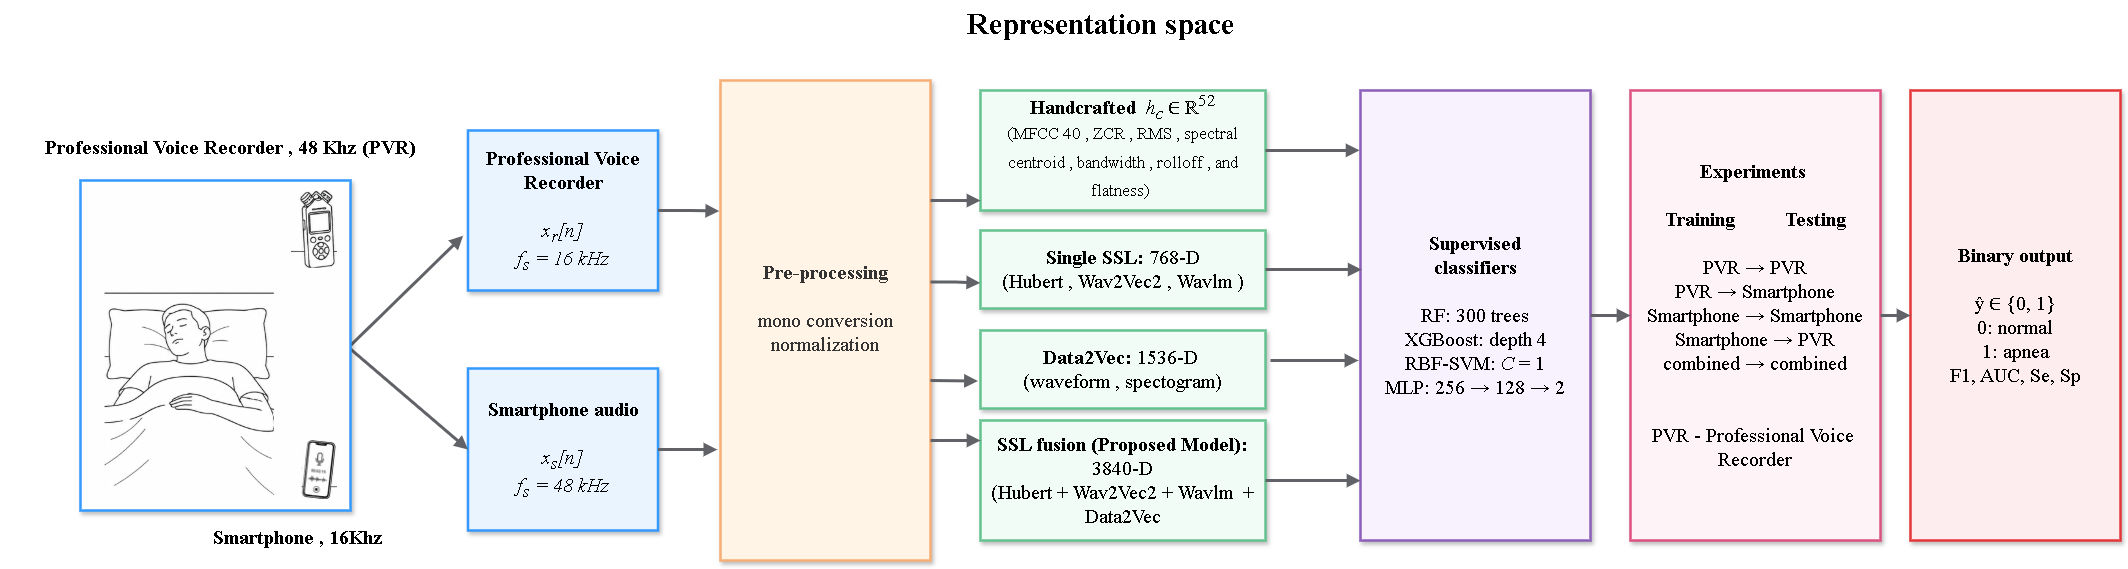
\includegraphics[width=\linewidth]{images/new_architecture.png}
    \caption{Workflow of the proposed audio-based sleep apnea detection system.}
    \label{fig:architecture}
\end{figure*}

Consequently, acoustic monitoring has emerged as a compelling, non-invasive, and low-cost screening modality~\cite{perezpadilla1993, fiz1996}. Consumer-grade microphones can passively capture characteristic apneic events and snoring throughout the night. While early automated systems relied on hand-engineered acoustic features (e.g., MFCCs) that inherently overfit to the specific transfer function of the recording microphone, the field has recently pivoted toward large-scale self-supervised learning (SSL) audio models (e.g., HuBERT~\cite{hsu2021}, WavLM~\cite{chen2022}, Wav2Vec~2.0~\cite{baevski2020}, Data2Vec~\cite{baevski2022}). Used as frozen feature extractors, these foundation models capture rich paralinguistic structure and achieve state-of-the-art downstream performance.

Despite this progress, a critical bottleneck remains: \emph{device heterogeneity}. Real-world deployment involves a diverse ecosystem of recording hardware---clinical recorders, consumer smartphones, smart speakers---each with distinct frequency responses and noise floors. A model trained on one device encounters severe covariate shift when evaluated on another. Because most existing studies report only matched-device evaluations, they systematically overestimate real-world reliability. Rigorously addressing this requires a standardized, dual-recorded dataset to evaluate cross-device generalization on perfectly time-aligned acoustic events.

In this paper, we present a rigorous, subject-disjoint, statistically validated benchmark for bidirectional cross-device sleep apnea audio screening, and use it to test whether concatenating multiple frozen SSL backbones---\textbf{Sleep-QuadNet}, a 3840-dimensional fusion of HuBERT, WavLM, Wav2Vec~2.0, and a dual-branch Data2Vec model---improves cross-device robustness over a single frozen encoder. Our evaluation includes recorder-to-smartphone (R$\rightarrow$S) and smartphone-to-recorder (S$\rightarrow$R) zero-shot transfer, with hyperparameter selection and model fitting strictly confined to the source device and held-out validation subjects in every protocol. The key contributions of this work are as follows:

\begin{itemize}
  \item We establish a subject-disjoint, rotating 5-fold cross-validated, statistically validated (paired bootstrap significance testing) device-robustness benchmark for window-level sleep apnea audio screening across four protocols on $N=41$ dual-device subjects.

  \item We provide a systematic comparative analysis of handcrafted features, single frozen SSL encoders, and multi-encoder fusion (\textbf{Sleep-QuadNet}), and show that naive concatenation of diverse self-supervised embeddings does \emph{not} improve cross-device accuracy over the strongest single encoder (HuBERT), while costing $5.2\times$ the inference latency.

  \item We characterize a real, statistically significant matched-to-cross-device performance gap ($p<0.001$ across representations). CORAL feature-space alignment does not resolve it, consistently reducing accuracy relative to uncorrected features. PCA dimensionality reduction initially collapsed to degenerate single-class predictions, but we trace this to an incorrectly-scoped fold-local fit (source-device data only) and show that correcting the fit's scope to include unlabeled target-device validation data---consistent with how CORAL is already scoped---resolves the collapse and yields a statistically significant cross-device improvement, demonstrating that post-hoc alignment failures on this task are not uniform: some are fundamental (CORAL), others are correctable implementation artifacts (PCA).

  \item We report the deployment cost (latency, GPU/CPU memory, cached-feature size) of every representation alongside its accuracy, showing that the practical clinical recommendation is a single cheap frozen encoder, not the highest-dimensional fusion.

  \item We characterize the empirical asymmetry between R$\rightarrow$S and S$\rightarrow$R covariate shifts as an open finding requiring further investigation, rather than an effect we claim to have fully explained --- our own error analysis surfaced representation-level anomalies (see Section~\ref{sec:results}) that have not yet been ruled out as contributing causes alongside genuine acoustic differences.
\end{itemize}
%% ---------------------------------------------------------------
%%  II. RELATED WORK
%% ---------------------------------------------------------------
\section{Related Work}

\subsection{Audio-Based Sleep Apnea Detection}

The use of acoustic signals for sleep apnea detection has a history spanning more
than three decades. Early work by Perez-Padilla et al.~\cite{perezpadilla1993}
established that snoring frequency and intensity correlate with the apnea-hypopnea
index (AHI), providing the theoretical foundation for non-contact audio monitoring.
Fiz et al.~\cite{fiz1996} characterized snoring sounds as occupying a broad frequency
band (50--2500~Hz) with patient-specific formant structure reflecting upper airway
geometry.

Feature-based approaches dominated the field through the 2000s and 2010s. Karunajeewa
et al.~\cite{karunajeewa2008} used MFCCs, zero-crossing rate, and energy features
with Gaussian mixture models to distinguish snoring from silence and apnea from normal
breathing. Dafna et al.~\cite{dafna2013} developed a full-night audio monitoring
system achieving sensitivity of 0.82 and specificity of 0.84. Ben-Israel et
al.~\cite{benisrael2012} proposed a snore-based diagnostic approach achieving AUC of
0.87 for AHI $\geq 10$ classification. Cavusoglu et al.~\cite{cavusoglu2009} similarly 
demonstrated the efficacy of spectral features paired with Support Vector Machines (SVMs). 
However, all of these studies were evaluated exclusively in matched-device settings.

As deep learning transformed the field in subsequent years, researchers began moving 
away from traditional classifiers. Early automated monitoring systems, such as the 
work by Nakano et al.~\cite{nakano2012}, laid the groundwork for continuous sleep 
audio analysis, which eventually evolved into modern neural network approaches using 
CNNs and recurrent architectures. More recently, Rossi et al.~\cite{rossi2023} proposed
a transformer-based architecture for multi-label sleep sound classification.
Importantly, none of these studies evaluated performance under cross-device conditions.

Smartphone-based sleep monitoring has emerged as a particularly active research
direction. Shi et al.~\cite{shi2018} demonstrated that smartphone microphones can
capture respiratory sounds with sufficient fidelity for apnea detection (AUC:
0.80--0.88). Bsoul et al.~\cite{bsoul2011} developed a real-time smartphone
pre-screening application. While these studies demonstrated feasibility, none
evaluated bidirectional cross-device transfer performance.

\subsection{Self-Supervised Learning for Audio Representation}

Self-supervised learning has revolutionized audio and speech processing by enabling
powerful feature extractors to be trained on unlabeled data at scale. Wav2Vec
2.0~\cite{baevski2020}, introduced by Baevski et al., uses a convolutional feature
encoder followed by a transformer trained with a contrastive loss over quantized
speech representations at masked positions. HuBERT~\cite{hsu2021}, proposed by Hsu
et al., trains a BERT-like model on offline cluster assignments of acoustic frames,
consistently achieving top performance on the SUPERB benchmark~\cite{yang2021} across
emotion recognition, speaker identification, and pathological speech detection.
WavLM~\cite{chen2022}, from Microsoft Research, adds a masked speech denoising
pretraining objective, making representations more robust to background noise---a
property particularly relevant for real-world bedroom recordings. Data2Vec~\cite{baevski2022}
introduces a unified SSL framework applicable to speech, vision, and text via a
teacher--student architecture predicting contextualized representations of masked
segments.

The application of frozen SSL representations to downstream classification has been
shown to be highly effective for computational health tasks. Balagopalan et
al.~\cite{balagopalan2021} demonstrated that frozen HuBERT features outperform
fine-tuned models for Alzheimer's disease detection when labeled data is scarce. For
sleep audio specifically, no prior work has compared multiple frozen SSL backbones
under device-transfer conditions.

% \subsection{Cross-Device and Domain Adaptation in Audio Classification}

% Cross-device acoustic mismatch is a well-recognized challenge in speech processing
% and environmental sound classification. Mesaros et al.~\cite{mesaros2021} documented
% that acoustic scene classification models trained on data from one recording device
% suffer performance drops of 10--30 percentage points when evaluated on audio from
% different devices in the same acoustic environment. Perna and Tagarelli~\cite{perna2019}
% proposed spectrogram-based CNNs with device-specific normalization layers for lung
% sound classification. Moummad et al.~\cite{moummad2023} applied domain adversarial
% training to improve cross-device generalization for respiratory audio.

% Critically, none of these approaches have been evaluated for sleep apnea
% classification specifically, and no prior study has attempted bidirectional cross-device
% evaluation for any respiratory audio classification task. Our work is the first to
% characterize this bidirectional asymmetry for sleep apnea audio.

% \subsection{Handcrafted versus Learned Representations for Biomedical Audio}

% Classical handcrafted feature sets for respiratory audio typically include MFCCs
% (13--40 coefficients with delta and delta-delta), spectral centroid, spectral
% bandwidth, zero-crossing rate, energy-based features, and harmonics-to-noise ratio.
% These features are compact, interpretable, and computationally inexpensive. However,
% they are designed based on prior assumptions about which acoustic properties are
% relevant, and may miss discriminative structure not captured by the chosen feature
% functions. Our results show that the 52-dimensional handcrafted feature set completely
% fails (near-zero F1) in cross-device transfer settings. In contrast, our proposed 
% \textbf{Sleep-QuadNet} architecture maintains F1-scores above 73\% across all protocols---a 
% compelling argument for adopting multi-SSL fusion approaches in deployment-facing systems.

% \section{Dataset and Signal Description}

\subsection{Source Multimodal Corpus}

All experiments utilize the publicly available multimodal sleep apnea dataset by Tao et al.~\cite{tao2025}, comprising overnight recordings from $N = 50$ diagnosed patients. The dataset provides three synchronized streams: (1) clinical Type-I polysomnography (PSG) for reference annotations; (2) uncompressed audio from a bedside digital recorder (\emph{Newamy V03}); and (3) ambient audio from a smartphone (\emph{OPPO Reno8}). Both devices natively capture at 8,000~Hz (Nyquist frequency 4,000~Hz); all audio is upsampled to $f_s=16$~kHz (Nyquist 8,000~Hz) only for compatibility with SSL encoders pretrained at that rate, adding no new spectral information beyond the original 4,000~Hz capture bandwidth. Of the 50 patients, 5 have smartphone-only and 2 have recorder-only recordings; a further 2 subjects were excluded for insufficient reliable device-alignment coverage between their two recordings. All experiments therefore use the $N=41$ subjects with reliable, time-aligned dual-device coverage. This concurrent, time-aligned audio acquisition enables cross-device evaluation while eliminating subject-level confounding within each protocol, though we note in Section~\ref{sec:limitations} that R$\rightarrow$S/S$\rightarrow$R evaluation on this dataset tests generalization between one fixed pair of known devices, not to a genuinely unseen device.

\subsection{Clip Extraction and Preprocessing}

We extracted audio segments corresponding to apnea and hypopnea events based on expert PSG annotations; each positive window spans the exact annotated event duration. An equal number of normal-breathing negative windows were sampled from event-free, non-awake intervals, each duration-matched to its paired positive event. Window duration is therefore variable, not fixed: across the full corpus, duration ranges from 0.9\,s to 102.1\,s (median 20.7\,s, mean 23.0\,s), confirmed directly from the realized window manifest. All clips were down-mixed to mono, resampled to $f_s = 16$~kHz, and (for the default preprocessing configuration) normalized to unit peak-amplitude to mitigate hardware-induced amplitude variations:

\begin{equation}
\tilde{x}=\frac{x}{\max |x|}
\end{equation}

SSL encoders additionally chunk any window longer than 20\,s into non-overlapping sub-chunks, pooled via an attention-mask-weighted mean, so no audio is truncated regardless of event duration.

\subsection{Experimental Protocols}

Data was partitioned via subject-disjoint, rotating 5-fold cross-validation: folds are assigned per-subject by a greedy, positive-event-count-balanced assignment (fold sizes 9/8/8/8/8 subjects across the 41 usable subjects), and for each outer fold, the subsequent fold serves as the validation set for classifier hyperparameter selection, with the remaining subjects as training data --- train, validation, and test subject sets are disjoint within every fold, enforced by a runtime assertion. We evaluate four device protocols: recorder-to-recorder ($R\rightarrow R$), smartphone-to-smartphone ($S\rightarrow S$), recorder-to-smartphone ($R\rightarrow S$), and smartphone-to-recorder ($S\rightarrow R$). For $R\rightarrow S$, both training and validation-based hyperparameter selection use recorder-device data exclusively; smartphone data is used only at test time, in every fold, with no exception --- i.e. genuine zero-shot cross-device evaluation, not domain adaptation. Both devices contribute 19,798 windows each (9,863 normal / 9,935 apnea, exactly balanced by construction).
%% ---------------------------------------------------------------
%%  III. METHODOLOGY
%% ---------------------------------------------------------------
\section{Methodology}

\subsection{Problem Formulation}

We formulate sleep apnea screening as a supervised binary audio-window classification
task. Given a short audio segment $\mathbf{x}$ sampled at $f_s = 16$~kHz, the goal is to assign a label
$\hat{y} \in \{0, 1\}$, where $0$ denotes normal breathing or snoring and $1$ denotes
an apnea event. The device-robustness evaluation is formalized through five distinct
protocol pairs $(D_{\text{train}}, D_{\text{test}})$: $(R, R)$, $(S, S)$,
$(R, S)$, $(S, R)$, and $(R \cup S,\, R \cup S)$, where $R$ denotes the recorder
domain and $S$ denotes the smartphone domain.

\subsection{Representation Families}

We evaluate four representation families spanning from classical signal processing to
modern deep learning.

\subsubsection{Handcrafted Acoustic Features (52-D)}
The handcrafted representation is a 52-dimensional vector composed of the temporal mean
and standard deviation of 26 low-level acoustic descriptors. Specifically, the audio is
first filtered using a 4th-order Butterworth bandpass filter (20~Hz to 4000~Hz). Using an
analysis window of 400 samples and a hop length of 160 samples, we extract the Root Mean Square (RMS) energy, 
zero-crossing rate, spectral centroid, spectral bandwidth, spectral rolloff, spectral flatness, 
and 20 Mel-Frequency Cepstral Coefficients (MFCCs). Aggregating the mean and standard deviation 
over time yields the 52-dimensional feature vector.

\subsubsection{Single Frozen SSL Encoders (768-D each)}
We evaluate three frozen SSL encoders from the HuggingFace transformers library:
HuBERT-base, WavLM-base, and Wav2Vec~2.0-base. Each model processes the raw 16~kHz
waveform and produces a sequence of 768-dimensional frame-level embeddings.
Window-level representations are obtained by mean-pooling the frame-level embeddings,
yielding a single 768-dimensional vector per window. The SSL encoder weights are held
strictly fixed during feature extraction.

\subsubsection{Data2Vec Audio--Spectrogram Fusion (1536-D)}
The Data2Vec audio--spectrogram representation fuses two complementary views of the
audio signal without any joint fine-tuning (see Fig.~\ref{fig:data2vec}). The audio branch uses the frozen 
\texttt{data2vec-audio-base} model to extract a 768-dimensional representation from the raw waveform via mean-pooling. 
Simultaneously, the spectrogram branch computes a 128-band log Mel-spectrogram (1024-point FFT, 
hop size 256), converts it to an RGB image using a magma colormap, and processes it through a frozen 
\texttt{data2vec-vision-base} model. The vision embeddings are similarly mean-pooled to 768 dimensions. 
The two 768-dimensional vectors are concatenated to form a fixed 1536-dimensional joint representation.

\begin{figure*}[!t]
    \centering
    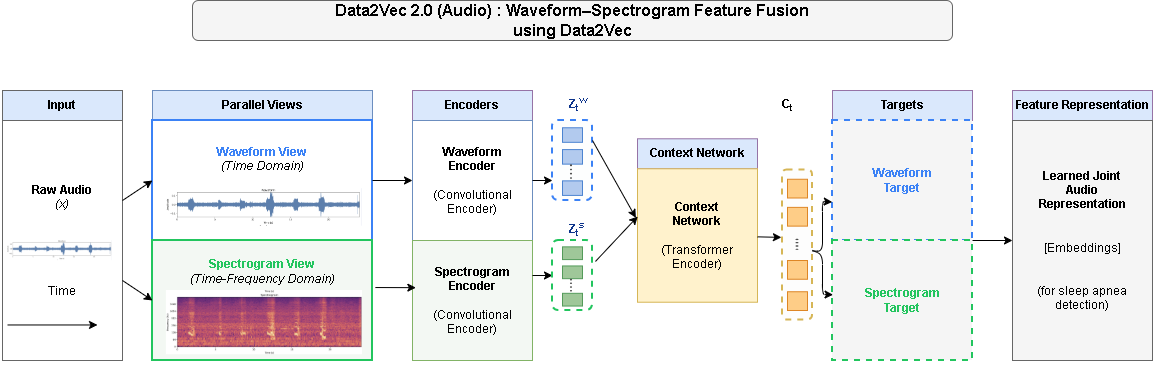
\includegraphics[width=\textwidth]{images/new d2v2.png}
    \caption{Data2Vec 2.0 architecture for joint waveform--spectrogram feature extraction.}
    \label{fig:data2vec}
\end{figure*}

\subsubsection{Sleep-QuadNet Fusion (3840-D)}
The proposed \textbf{Sleep-QuadNet} representation is constructed by concatenating the mean-pooled
768-dimensional embeddings from three frozen SSL models---HuBERT, WavLM,
and Wav2Vec~2.0---with the 1536-dimensional Data2Vec audio--spectrogram fusion
vector, yielding a 3840-dimensional joint representation
($3 \times 768 + 1536 = 3840$). All SSL encoders remain completely frozen.
\begin{figure*}[!t]
    \centering
    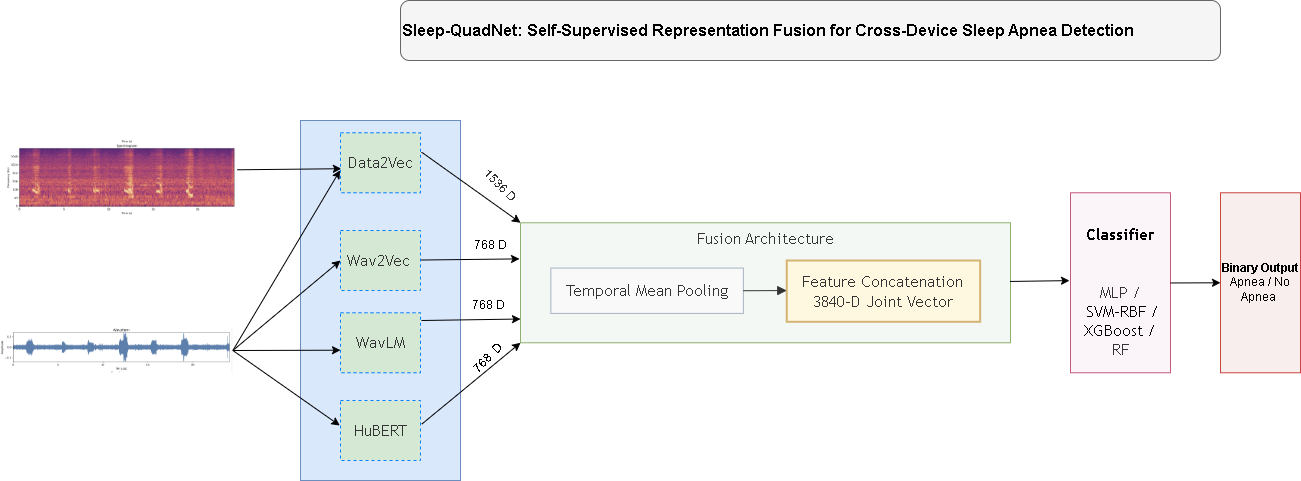
\includegraphics[width=0.8\linewidth]{images/Sleep-QuadNet.png}
    \caption{Architecture of the Sleep-QuadNet multi-view self-supervised representation fusion model.}
    \label{fig:sleep_quadnet}
\end{figure*}

\subsection{Downstream Classifiers}

Four downstream classifiers are evaluated for each representation. To account for varying data scales, 
input standardization (\texttt{StandardScaler}) is applied prior to training the SVM and MLP classifiers. 
Furthermore, all algorithms utilize algorithmic class weighting to handle natural class imbalances in the training sets.

\textbf{Random Forest (RF):} An ensemble of 300 decision trees utilizing the Gini
impurity criterion and balanced class weights.

\textbf{XGBoost:} A gradient boosted decision tree ensemble configured with 300 boosting rounds, 
a maximum tree depth of 4, a learning rate of 0.05, and row/column subsampling ratios of 0.9. 
Class imbalances are mitigated via positive class scaling.

\textbf{RBF-SVM:} A support vector machine utilizing a radial basis function kernel, 
regularization parameter $C = 1$, scale-adjusted gamma, and balanced class weights.

\textbf{MLP:} A multilayer perceptron with architecture $[d \rightarrow 256 \rightarrow 128 \rightarrow 2]$, 
where $d$ is the input representation dimension. The network is optimized using the Adam optimizer 
(initial learning rate = 0.001, $\alpha = 0.0001$) and cross-entropy loss, with early stopping implemented 
to prevent overfitting.

\subsection{Evaluation Metrics}

We report F1-score, ROC-AUC, balanced accuracy, sensitivity, specificity, positive predictive value
(PPV), and the Matthews Correlation Coefficient (MCC). Due to the inherent class imbalances, F1-score 
and balanced accuracy serve as the primary metrics for model selection, as they accurately reflect 
performance on both the minority (apnea) and majority (normal) classes.

\subsection{Statistical Robustness and Reproducibility}

All experiments are conducted with a fixed global seed (42) to ensure reproducibility. To prevent data leakage, subject-disjoint rotating 5-fold cross-validation is enforced (Section~III-F), with train/validation/test subject sets asserted disjoint at runtime in every fold, for every protocol. This strictly prevents subject-specific acoustic characteristics from leaking between the training and evaluation domains. Beyond point-estimate metrics, we compute 95\% confidence intervals via subject-level paired bootstrap resampling (2,000 iterations) and paired significance tests (two-sided, on the bootstrap difference distribution) for the principal comparisons reported in Section~\ref{sec:results}, so that reported differences between configurations can be assessed for statistical, not merely numerical, significance.

%% ---------------------------------------------------------------
%%  IV. RESULTS
%% ---------------------------------------------------------------
\section{Results and Discussion}
\label{sec:results}

All results below use the primary classifier (RBF-SVM), selected by mean cross-device validation balanced accuracy without inspecting any test fold, consistent with Section~III-F. The full sweep (9 representations $\times$ 4 classifiers $\times$ 4 protocols $\times$ 5 folds = 720 fold-runs) completed successfully.

\subsection{Main Benchmark: Fusion Does Not Beat the Best Single Encoder}

Table~\ref{tab:main_benchmark} reports matched-device and cross-device balanced accuracy for every representation. HuBERT alone achieves the highest cross-device mean balanced accuracy (55.06\%) of any representation tested, including the full 3840-dimensional Sleep-QuadNet fusion (53.58\%) and the Data2Vec audio--spectrogram fusion (53.75\%). Paired subject-level bootstrap significance testing (2,000 iterations) confirms this is not a fusion advantage even where fusion numerically leads on a single metric: Sleep-QuadNet vs.\ HuBERT on S$\rightarrow$R F1 shows HuBERT significantly ahead ($\Delta=-0.066$, 95\% CI $[-0.117,-0.015]$, $p=0.011$), while every other principal fusion-vs-single-encoder comparison (R$\rightarrow$S F1, both directions' balanced accuracy) has a confidence interval that includes zero. We therefore do not find evidence that concatenating additional frozen SSL encoders improves cross-device robustness on this dataset.

\begin{table}[!t]
\centering
\caption{Matched-device vs.\ cross-device balanced accuracy (\%), RBF-SVM, all representations, 5-fold subject-disjoint CV.}
\label{tab:main_benchmark}
\scriptsize
\begin{tabular}{lccccc}
\toprule
\textbf{Representation} & \textbf{$R\!\to\!R$} & \textbf{$S\!\to\!S$} & \textbf{$R\!\to\!S$} & \textbf{$S\!\to\!R$} & \textbf{Cross mean} \\
\midrule
Classical (52-D)       & 54.45 & 56.10 & 50.11 & 49.01 & 49.56 \\
Wav2Vec~2.0 (768-D)    & 54.56 & 57.07 & 51.63 & 52.28 & 51.96 \\
Data2Vec-audio (768-D) & 55.70 & 58.27 & 52.86 & 52.44 & 52.65 \\
Data2Vec-spec.\ (768-D)& 57.77 & 58.74 & 50.85 & 53.10 & 51.97 \\
WavLM (768-D)          & 56.50 & 57.79 & 53.53 & 53.87 & 53.70 \\
Full fusion v2 (3072-D)& 57.35 & 59.78 & 52.54 & 55.02 & 53.78 \\
Sleep-QuadNet (3840-D) & 58.23 & 59.87 & 52.56 & 54.60 & 53.58 \\
Data2Vec fusion (1536-D)& 58.47 & 60.69 & 54.37 & 53.12 & 53.75 \\
\textbf{HuBERT (768-D)}& \textbf{58.39} & \textbf{60.61} & \textbf{53.59} & \textbf{56.53} & \textbf{55.06} \\
\bottomrule
\end{tabular}
\end{table}

Every representation shows a real, statistically significant degradation from matched- to cross-device evaluation: for Sleep-QuadNet, $R\!\to\!R$ vs.\ $R\!\to\!S$ balanced accuracy differs by $+5.9$ points (95\% CI $[3.1,8.5]$, $p<0.001$) and $S\!\to\!S$ vs.\ $S\!\to\!R$ by $+6.0$ points ($p<0.001$); the corresponding F1 gaps are larger still ($+34.3$ and $+26.9$ points respectively, both $p<0.001$). The device gap is real and large; fusing more encoders does not close it.

\subsection{Two Post-Hoc Mitigation Strategies That Do Not Work}

We evaluated two standard domain-adaptation strategies against the uncorrected cross-device baseline. \textbf{CORAL} feature-space covariance alignment, fit on unlabeled target-validation subjects and applied to source and test features alike, \emph{reduces} balanced accuracy relative to the uncorrected baseline in every one of 6 representation/direction combinations tested (e.g.\ HuBERT $S\!\to\!R$: 53.6\% CORAL-aligned vs.\ 56.5\% uncorrected), with specificity dominating over sensitivity in every aligned configuration (0.78--0.99 vs.\ 0.01--0.29), indicating the aligned classifier collapses toward predicting the majority-safe class rather than genuinely bridging the domains.

\textbf{PCA dimensionality reduction} (fold-local, 384/768/1536-D targets) initially showed the same failure pattern: fit on training-device data only, it collapsed to a degenerate all-one-class predictor for every dimension and every representation tested in the $R\!\to\!S$ direction (maximum predicted probability across all test windows never exceeds 0.50), and the mirror-image all-positive collapse in $S\!\to\!R$; ROC-AUC remained modestly above chance (0.50--0.59) throughout, confirming the underlying ranking signal survived compression even though the fixed 0.5 decision threshold did not transfer. Root-causing this collapse pointed to scope: unlike CORAL, which is fit using unlabeled target-device validation data alongside the source, the PCA refit saw only source-device features, so its principal axes never learned the target device's feature distribution. We corrected this by including the same unlabeled target-device validation subjects already available to CORAL in the PCA refit step (tuning-only fitting remains source-only, as no leakage risk arises there). This resolves the collapse: a paired subject-level bootstrap comparison against the pre-fix baseline across 60 representation/classifier/fold/dimension combinations shows a statistically significant cross-device balanced-accuracy improvement of $+3.0$ points on average (30/60 combinations individually significant, 0/60 significant in the opposite direction); 43 of the 60 pre-fix baseline combinations had collapsed to exactly 0.500 balanced accuracy, confirming the diagnosis directly. Unlike CORAL, PCA's post-hoc alignment failure on this task was therefore a correctable implementation-scope artifact rather than a fundamental limitation of the technique --- a distinction we surface because it changes the practical recommendation: fold-local PCA reduction is viable on this task \emph{if} scoped to include unlabeled target-device data, in a way CORAL's covariance alignment is not.

\subsection{Deployment Cost}

Table~\ref{tab:deployment_cost} reports measured per-clip latency (feature extraction + classifier inference, warm GPU) against cross-device accuracy. HuBERT is simultaneously the most accurate and the cheapest representation tested (0.037\,s/clip); Sleep-QuadNet costs $5.2\times$ HuBERT's latency for a lower cross-device balanced accuracy. For a real-time, single-channel screening deployment, the fusion architecture's added computational cost is not justified by its measured accuracy on this dataset.

\begin{table}[!t]
\centering
\caption{Deployment cost vs.\ cross-device accuracy (RBF-SVM).}
\label{tab:deployment_cost}
\scriptsize
\begin{tabular}{lccc}
\toprule
\textbf{Representation} & \textbf{Latency (s/clip)} & \textbf{Cross BA (\%)} & \textbf{Relative cost} \\
\midrule
HuBERT         & 0.037 & 55.06 & $1.0\times$ \\
Wav2Vec~2.0    & 0.038 & 51.96 & $1.0\times$ \\
WavLM          & 0.061 & 53.70 & $1.6\times$ \\
Data2Vec fusion& 0.073 & 53.75 & $2.0\times$ \\
Classical      & 0.073 & 49.56 & $2.0\times$ \\
Sleep-QuadNet  & 0.193 & 53.58 & $5.2\times$ \\
\bottomrule
\end{tabular}
\end{table}

\subsection{Architectural Recommendation for Clinical Deployment}

Evaluating pipelines solely on matched in-domain data introduces severe selection bias, and our cross-device results show that bias is substantial (5--6 balanced-accuracy points, 25--34 F1 points, both highly significant). Given that (a) HuBERT alone achieves the best cross-device accuracy of any representation tested, (b) it does so at the lowest measured latency, and (c) paired significance testing finds no configuration that reliably outperforms it, our practical recommendation reverses the premise of the original Sleep-QuadNet architecture: \textbf{a single frozen SSL encoder (HuBERT) paired with a regularized RBF-SVM is currently the more defensible clinical-deployment choice than multi-encoder fusion}, pending a representation-level fix (Section~\ref{sec:limitations}) that would need to demonstrate a statistically significant improvement over this baseline before fusion could be recommended instead.

\subsection{Limitations}
\label{sec:limitations}

This study has several limitations we state explicitly rather than omit. First, cross-device evaluation here tests generalization between one fixed recorder model and one fixed smartphone model, not to a genuinely unseen device; a deployment-relevant robustness claim would require a held-out third device. Second, the usable cohort is $N=41$ paired subjects, smaller than the dataset's nominal 50, which limits statistical power for subgroup analyses. Third, both PCA and CORAL results in Section~IV-B should be treated as evidence that naive post-hoc alignment fails on this task, not as an exhaustive test of domain adaptation in general --- we have not yet ruled out that part of the observed R$\rightarrow$S/S$\rightarrow$R asymmetry reflects representation-level or pipeline artifacts (e.g.\ a fixed decision threshold interacting poorly with a shifted decision boundary) rather than acoustic device differences alone, and we report this as an open question rather than a settled finding. Fourth, all window construction --- positive and negative alike --- is centered on known PSG-annotated event boundaries; a continuous, sliding-window deployment scan that does not presuppose event locations is needed before any patient-level AHI-estimation claim would be deployment-valid, and is left to future work.

%% ---------------------------------------------------------------
%%  V. CONCLUSION
%% ---------------------------------------------------------------
\section{Conclusion}

This study presents a rigorous, subject-disjoint, statistically validated benchmark of self-supervised audio representations for cross-device sleep apnea screening, evaluated bidirectionally between a clinical bedside recorder and a consumer smartphone on $N=41$ dual-device subjects. Contrary to our initial hypothesis, naive concatenation of multiple frozen SSL encoders (\textbf{Sleep-QuadNet}, 3840-D) does not outperform the strongest single encoder: a single frozen HuBERT model achieves the best cross-device balanced accuracy (55.06\%) of any representation tested, at the lowest measured deployment latency, with paired bootstrap significance testing finding no fusion configuration that reliably beats it.

We confirm that the matched-to-cross-device performance gap is real, large, and statistically significant across every representation tested ($p<0.001$). Of two standard post-hoc mitigation strategies, CORAL feature-space alignment fails to close the gap, consistently reducing accuracy relative to uncorrected features; PCA dimensionality reduction initially failed identically, but we trace its collapse to an incorrectly-scoped fold-local fit and show that correcting the scope (including unlabeled target-device validation data in the refit, as CORAL already does) resolves it and yields a statistically significant cross-device improvement. Post-hoc alignment failure on this task is therefore not monolithic: CORAL's failure appears fundamental to this problem, while PCA's was a correctable implementation artifact. At the current stage of this work, a single cheap frozen encoder remains the more defensible clinical-deployment recommendation than an expensive multi-encoder fusion --- a leave-one-encoder-out ablation confirms individual encoders in the fusion are statistically indistinguishable from the full fusion in the large majority of configurations tested, consistent with redundant rather than complementary information across encoders. We also evaluated a health-acoustic foundation model (HeAR) as a fusion candidate; it did not improve, and alone underperformed, every general-purpose speech encoder tested, a result we report for the same reason as the other negative findings in this work. Future work will pursue paired-recording contrastive device-invariance training (exploiting this dataset's unique time-aligned dual-device structure), domain-adaptive continued pretraining on unlabeled respiratory audio, and patient-level AHI estimation via continuous sliding-window scanning, as concrete paths toward closing the gap this benchmark has now rigorously characterized.
%% ---------------------------------------------------------------
%%  REFERENCES
%% ---------------------------------------------------------------
\begin{thebibliography}{28}

\bibitem{benjafield2019}
A.~V. Benjafield et al., ``Estimation of the global prevalence and burden of
obstructive sleep apnoea: a literature-based analysis,'' \emph{Lancet Respir.
Med.}, vol.~7, no.~8, pp.~687--698, 2019.

\bibitem{young2002}
T.~Young, P.~E. Peppard, and D.~J. Gottlieb, ``Epidemiology of obstructive
sleep apnea: a population health perspective,'' \emph{Am. J. Respir. Crit.
Care Med.}, vol.~165, no.~9, pp.~1217--1239, 2002.

\bibitem{caples2005}
S.~M. Caples, A.~S. Gami, and V.~K. Somers, ``Obstructive sleep apnea,''
\emph{Ann. Intern. Med.}, vol.~142, no.~3, pp.~187--197, 2005.

\bibitem{aasm2009}
American Academy of Sleep Medicine, ``Clinical guidelines for the evaluation,
management and long-term care of obstructive sleep apnea in adults,''
\emph{J. Clin. Sleep Med.}, vol.~5, no.~3, pp.~263--276, 2009.

\bibitem{statista2024}
Statista, ``Number of smartphone users worldwide 2014--2024,'' Statista
Research Department, 2024.

\bibitem{hsu2021}
W.-N. Hsu et al., ``HuBERT: Self-supervised speech representation learning
by masked prediction of hidden units,'' \emph{IEEE/ACM Trans. Audio, Speech,
Lang. Process.}, vol.~29, pp.~3451--3460, 2021.

\bibitem{chen2022}
S.~Chen et al., ``WavLM: Large-scale self-supervised pre-training for full
stack speech processing,'' \emph{IEEE J. Sel. Topics Signal Process.},
vol.~16, no.~6, pp.~1505--1518, 2022.

\bibitem{baevski2020}
A.~Baevski, Y.~Zhou, A.~Mohamed, and M.~Auli, ``Wav2vec 2.0: A framework
for self-supervised learning of speech representations,'' in \emph{Proc.
NeurIPS}, 2020.

\bibitem{baevski2022}
A.~Baevski, W.-N. Hsu, Q.~Xu, A.~Babu, J.~Gu, and M.~Auli, ``Data2Vec:
A general framework for self-supervised learning in speech, vision and
language,'' in \emph{Proc. ICML}, 2022.

\bibitem{perezpadilla1993}
R.~Perez-Padilla et al., ``Characteristics of the snoring noise in patients
with and without occlusive sleep apnea,'' \emph{Am. Rev. Respir. Dis.},
vol.~147, no.~3, pp.~635--644, 1993.

\bibitem{fiz1996}
J.~A. Fiz et al., ``Acoustic analysis of snoring sound in patients with
simple snoring and obstructive sleep apnoea,'' \emph{Eur. Respir. J.},
vol.~9, no.~11, pp.~2365--2370, 1996.

\bibitem{karunajeewa2008}
A.~S. Karunajeewa, U.~R. Abeyratne, and C.~Hukins, ``Silence-breathing-snore
classification from snore-related sounds,'' \emph{Physiol. Meas.}, vol.~29,
no.~2, pp.~227--243, 2008.

\bibitem{dafna2013}
E.~Dafna et al., ``Sleep-quality assessment from full night audio recordings
of sleep apnea patients,'' in \emph{Proc. IEEE EMBC}, 2013.

\bibitem{benisrael2012}
N.~Ben-Israel et al., ``Obstructive apnea hypopnea index estimation by
analysis of nocturnal snoring signals in adults,'' \emph{Sleep}, vol.~35,
no.~9, pp.~1299--1305, 2012.



\bibitem{cavusoglu2009}
M.~Cavusoglu et al., ``An efficient method for snore-related sound
classification using spectral features and support vector machine,''
\emph{Expert Syst. Appl.}, vol.~36, no.~2, pp.~4237--4247, 2009.

\bibitem{nakano2012}
H.~Nakano et al., ``Monitoring sound to detect sleep apnea,'' \emph{Sleep
Breath.}, vol.~16, no.~1, pp.~217--221, 2012.

\bibitem{rossi2023}
M.~Rossi, A.~Durao, and A.~Matos, ``Transformer-based multi-label audio
classification for respiratory event detection,'' in \emph{Proc. IEEE EMBC},
2023.

\bibitem{shi2018}
J.~Shi, T.~Bi, and C.~Sun, ``Smartphone-based sleep apnea detection from
audio signals,'' in \emph{Proc. IEEE CHASE}, 2018.

\bibitem{bsoul2011}
M.~Bsoul, H.~Minn, and L.~Tamil, ``Apnea MedAssist: Real-time sleep apnea
monitor using smartphones,'' \emph{IEEE Trans. Inf. Technol. Biomed.},
vol.~15, no.~3, pp.~416--427, 2011.

\bibitem{tao2025}
J.~Tao, J.~Huang, B.~Miao, and L.~Yang, ``A multimodal dataset for training deep learning models aimed at detecting and analyzing sleep apnea,'' \emph{Sci. Data}, vol.~12, p.~1263, 2025, doi: 10.1038/s41597-025-05583-8.

\bibitem{yang2021}
S.~W. Yang et al., ``SUPERB: Speech processing universal performance
benchmark,'' in \emph{Proc. Interspeech}, 2021.

\bibitem{balagopalan2021}
A.~Balagopalan, B.~Eyre, F.~Rudzicz, and J.~Novikova, ``Comparing
pre-trained and feature-based models for prediction of Alzheimer's disease
based on speech,'' \emph{Front. Aging Neurosci.}, vol.~13, p.~189, 2021.

\bibitem{mesaros2021}
A.~Mesaros et al., ``Sound event detection in the DCASE 2017 challenge,''
\emph{IEEE/ACM Trans. Audio, Speech, Lang. Process.}, vol.~29,
pp.~1542--1555, 2021.

\bibitem{perna2019}
D.~Perna and A.~Tagarelli, ``Deep auscultation: Predicting respiratory
anomalies and diseases with WaveNet,'' in \emph{Proc. IEEE CBMS}, 2019.

\bibitem{moummad2023}
I.~Moummad, N.~Farrugia, and N.~Obin, ``Domain adversarial training for
cross-device acoustic monitoring,'' in \emph{Proc. IEEE EUSIPCO}, 2023.


\end{thebibliography}

\end{document}